<<<<<<< HEAD
\documentclass[11pt]{article}

\usepackage{graphicx}
\usepackage{lipsum}

\graphicspath{{./pictures/}}

\begin{document}
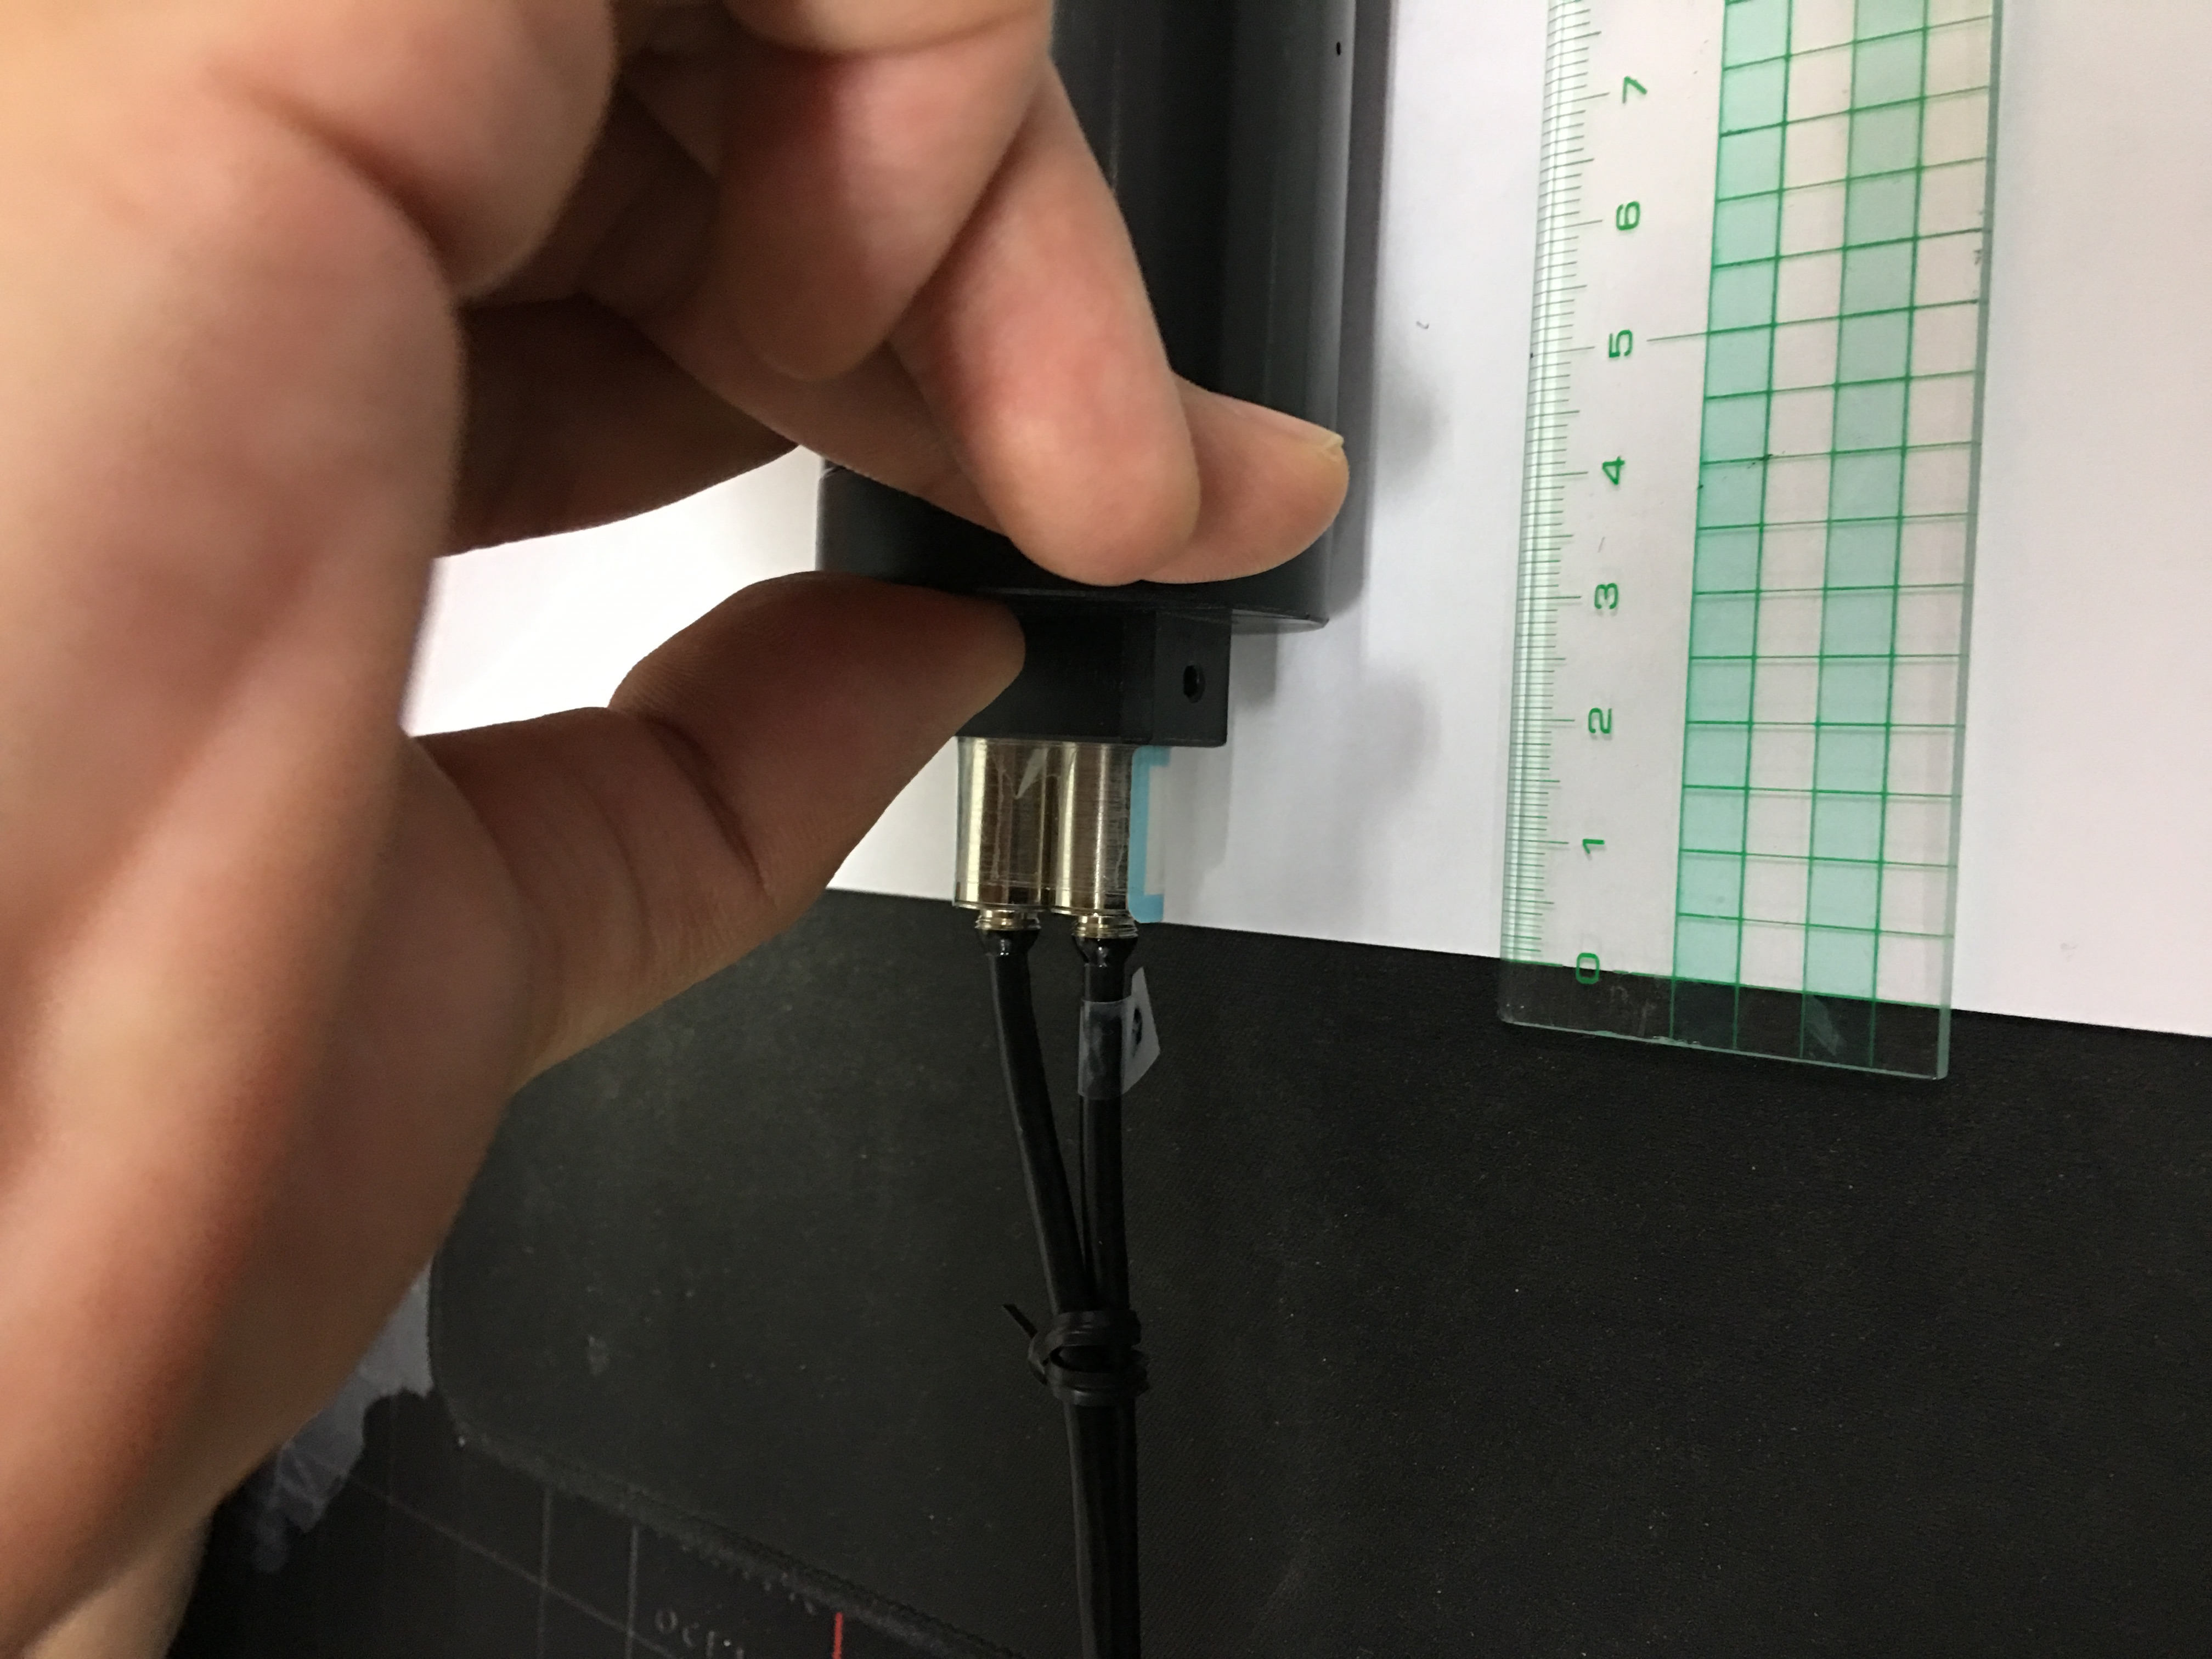
\includegraphics[width=0.8\textwidth]{img01.jpg}
%
\includegraphics[width=0.8\textwidth, page={3}]{RedVelvet.pdf}

\lipsum
=======
%\documentclass[11pt]{article}
\documentclass[footnote]{oblivoir}

\usepackage{mathtools}
\usepackage{amssymb} %% amsmath와 amssymb는 mathspec 이전
\usepackage{amsthm}
\usepackage{amsmath}
%\usepackage[MnSymbol]{mathspec}  %% kotex 이전
\usepackage{kotex}
\usepackage{bbm}

\theoremstyle{definition}
\newtheorem{thm}{정리}[section]
\newtheorem{defn}[thm]{정의}

\allowdisplaybreaks

\newcommand{\bZ}{{\mathbb{Z}}}
\newcommand{\norm}[1]{{\left \Vert #1 \right \Vert}}

\begin{document}
hello world! $f(x)$

\[\int_{a}^b f(x)dx \]

\begin{equation}
\int_{a}^b f(x)dx
\end{equation}

$P_1$\을 재화1의 가격이라고 하고, $P_2$\를 재화 2의 가격이라 하자. 소비자가 사용할 수 있는 예산의 한도가 $m$원까지일 때, 생각할 수 있는 제약모델은 다음과 같다:

\begin{equation}
p_1 x_1 + p_2 x_2 \leq m.
\end{equation}

자주 사용되는 효용함수로 \textbf{Cobb-Douglas} 효용함수가 있다. 이 함수의 정의는 다음과 같다:
\[u(x_1, x_2) = x_1^c x_2^d\]

$\int_a^b f(x)dx$

\[ \int_{a}^b f(x)dx \]

\begin{equation}
\int_{a}^b f(x)dx
\end{equation}

\begin{equation}
f(x) \hspace{4cm} g(x)
\end{equation}

\begin{equation}
a^x+y = a^x a^y
\end{equation}

\begin{equation*}
a^{x+y} = a^x a^y
\end{equation*}

\[
a^{x+y} = a^x a^y
\]

\[\begin{matrix}
A & B & C \\
d & e & f \\
1 & 2 & 3 \\
\end{matrix}\]

\[\begin{pmatrix}
A & B & C \\
d & e & f \\
1 & 2 & 3 \\
\end{pmatrix}\]

\[\begin{bmatrix}
A & B & C \\
d & e & f \\
1 & 2 & 3 \\
\end{bmatrix}\]


$\underset{under}{baseline}$ \\

$\overset{over}{baseline}$

\[
\sum_{\substack{1\leq i\leq p \\
1 \leq j \leq q \\
1 \leq k \leq r}}
a_{ij} b_{jk} c_{ki}
\]

\section{Hi}
\begin{thm}
\[ A=\{ x \in \mathbb{R} | x^2=a, \text{where $a$ is positive}\}\]
\end{thm}
\begin{proof}
ABC
\end{proof}

\section{Hello}
\begin{defn} \label{thm:1}
$\mathbb{R}$ is the set of all real numbers.
\end{defn}
\begin{proof}[증명]
DEF
\[ ABC \qedhere \]
\end{proof}

정리 \ref{thm:1}에 의해서

Note that
\begin{equation} \label{eq:1}
A \leq B
\end{equation}
and
\begin{equation} \label{eq:2}
B \leq A.
\end{equation}
So by (\ref{eq:1}) abd \eqref{eq:2}, we conclude that $A=B$.

\begin{equation}
\begin{split}
Hf(x)&=\mathrm{p.v.}\frac{1}{\pi}\int_{\mathbb{R}} \frac{f(y)}{x-y}dy\\
&=\lim_{\varepsilon \rightarrow 0}\frac{1}{\pi} \int_{|x-y|>\varepsilon}\frac{f(y)}{x-y}dy
\end{split}
\end{equation}

\begin{equation}
\begin{aligned}
Hf(x)&=\mathrm{p.v.}\frac{1}{\pi}\int_{\mathbb{R}} \frac{f(y)}{x-y}dy\\
&=\lim_{\varepsilon \rightarrow 0}\frac{1}{\pi} \int_{|x-y|>\varepsilon}\frac{f(y)}{x-y}dy
\end{aligned}
\end{equation}

\begin{align}
Hf(x)&=\mathrm{p.v.}\frac{1}{\pi}\int_{\mathbb{R}} \frac{f(y)}{x-y}dy\\
&=\lim_{\varepsilon \rightarrow 0}\frac{1}{\pi} \int_{|x-y|>\varepsilon}\frac{f(y)}{x-y}dy
\end{align}

\begin{align}
Hf(x)&=\mathrm{p.v.}\frac{1}{\pi}\int_{\mathbb{R}} \frac{f(y)}{x-y}dy\\
&=\lim_{\varepsilon \rightarrow 0}\frac{1}{\pi} \int_{|x-y|>\varepsilon}\frac{f(y)}{x-y}dy \nonumber
\end{align}

\begin{align*}
Hf(x)&=\mathrm{p.v.}\frac{1}{\pi}\int_{\mathbb{R}} \frac{f(y)}{x-y}dy\\
&=\lim_{\varepsilon \rightarrow 0}\frac{1}{\pi} \int_{|x-y|>\varepsilon}\frac{f(y)}{x-y}dy
\end{align*}

Cobb-Douglas 모델의 MRS(Marginal rate of substitution)\를 구해보도록 하자.
$u(x_1, x_2)=x_1^c x_2^c$이라 할때,
\begin{align*}
\mathrm{RMS}&=-\frac{\partial u(x_1,x_2)/ \partial x_1}{\partial u (x_1, x_2) / \partial x_2}\\
&=-\frac{cx_1^{c-1} x_2^{d}}{dx_1^c x_2^{d-1}} \\
&=-\frac{cx_2}{dx_1}
\end{align*}
와 같다.

\begin{align*}
a_{11}& = b_{11}&
a_{12}& = b_{12}\\
a_{21}& = b_{21}&
a_{22}& = b_{22}+c_{22}
\end{align*}

\begin{flalign*}
a_{11}& = b_{11}&
a_{12}& = b_{12}\\
a_{21}& = b_{21}&
a_{22}& = b_{22} + c_{22}
\end{flalign*}

align환경이면서 한 행에 부연설명을 하고자 할 때 적합한 환경이다.
\begin{alignat}{2} %영역을 크게 두 개로 나눔
x& = y_1 - y_2 + y_3 - y_5 + y_8 - \dots &\quad& \text{by }\\
& = y' \circ y^* && \text{by } \\
& = y(0) y' && \text {by Axiom 1.}
\end{alignat}

$\mathbbm{1}$

$\mathbbm{ABCdef12}$

$\mathbbm{ABCdef12}$

$\mathcal{ABC}$

%$\mathscr{ABC}$

%$\mathds{ABC1}$

%$\mathfrack{ABCdef123}$

$\mathbb{Z}$

$\bZ$

$\norm{f}$

\[ \norm{\int_a^b f(x)} \]

$f\in L^p(\mathbb{R}) (1<p<\infty)$에 대하여 \[ Hf(x) = \mathrm{p.v} \int_{\mathbb{R}} \frac{f(y)}{\pi (x-y)dy}  \]
와 같이 정의한 변환을 힐버트 변환이라 한다. \\

$f\in L^p(\mathbb{R}) (1<p<\infty)$에 대하여

\[Hf(x) = \mathrm{p.v} \int_{\mathbb{R}} \frac{f(y)}{\pi (x-y)dy}  \]

와 같이 정의한 변환을 힐버트 변환이라 한다.

\[ \sum_{n=1}^\infty |a_n b_n| \leq \left( \sum_{n=1}^\infty |a_n|^p \right)^{\frac{1}{p}} \left(\sum_{n=1}^\infty |b_n|^q \right)^{\frac{1}{q}}
\]

$f\in {L^1(\mathbb{R}^d)}$이라는 것은 $\displaystyle \int_{\mathbb{R}^d} |f(x)|dx <\infty$일 때를 말한다.

\[
\begin{pmatrix*}[r]
-2 & 3\\
1  & -2
\end{pmatrix*}
\]


>>>>>>> 72a4c91614c5923a4d6ccb389a2c84a740b35839

\end{document}